\RequirePackage{ifpdf}
%\documentclass[journal]{vgtc}                % final (journal style)
\documentclass[review,journal]{vgtc}         % review (journal style)
%\documentclass[widereview]{vgtc}             % wide-spaced review
%\documentclass[preprint,journal]{vgtc}       % preprint (journal style)
%\documentclass[electronic,journal]{vgtc}     % electronic version, journal

%% Uncomment one of the lines above depending on where your paper is
%% in the conference process. ``review'' and ``widereview'' are for review
%% submission, ``preprint'' is for pre-publication, and the final version
%% doesn't use a specific qualifier. Further, ``electronic'' includes
%% hyperreferences for more convenient online viewing.

%% Please use one of the ``review'' options in combination with the
%% assigned online id (see below) ONLY if your paper uses a double blind
%% review process. Some conferences, like IEEE Vis and InfoVis, have NOT
%% in the past.

%% Please note that the use of figures other than the optional teaser is not permitted on the first page
%% of the journal version.  Figures should begin on the second page and be
%% in CMYK or Grey scale format, otherwise, colour shifting may occur
%% during the printing process.  Papers submitted with figures other than the optional teaser on the
%% first page will be refused.
%\begin{figure}[htb]
%	\centering
%	\fbox{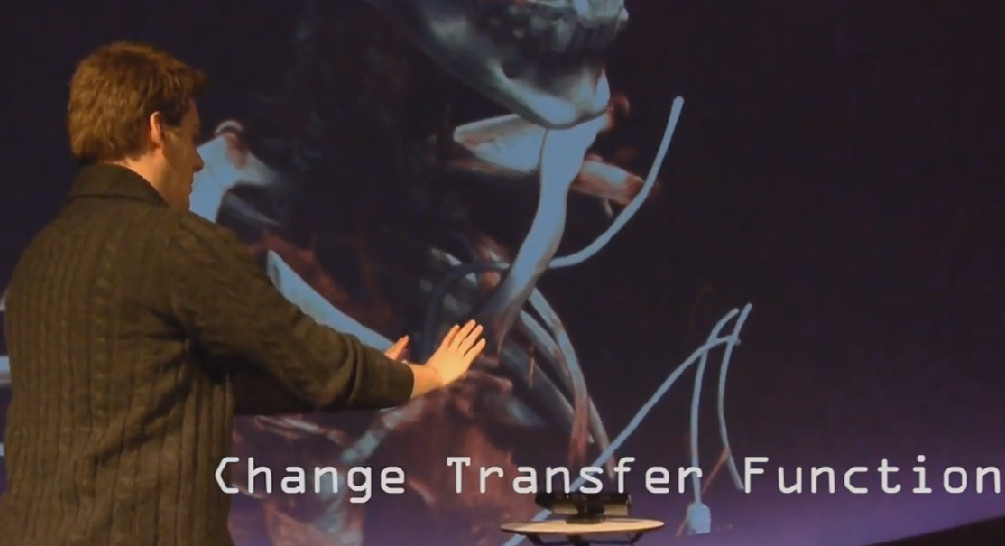
\includegraphics[width=1.0\linewidth]{images/dome_tf_change}}
%	\caption{Dome Closeup}
%	\label{img:dome_tf_change}
%\end{figure}

%% These three lines bring in essential packages: ``mathptmx'' for Type 1
%% typefaces, ``graphicx'' for inclusion of EPS figures. and ``times''
%% for proper handling of the times font family.

\usepackage{mathptmx}
\usepackage{graphicx}
\usepackage{times}
\usepackage{amsmath}
\usepackage{flushend}
\usepackage{subfigure}
\usepackage[noabbrev]{cleveref}
\usepackage{color}
%\usepackage[caption=false]{subfig}
\setlength{\fboxsep}{0pt}
\newcommand{\todo}[1]{\textbf{\textcolor{red}{[TODO: {#1}]}}}

%% We encourage the use of mathptmx for consistent usage of times font
%% throughout the proceedings. However, if you encounter conflicts
%% with other math-related packages, you may want to disable it.

%% This turns references into clickable hyperlinks.
%%\usepackage[bookmarks,backref=true,linkcolor=black]{hyperref} %,colorlinks
%%\hypersetup{
%%  pdfauthor = {},
%%  pdftitle = {},
%%  pdfsubject = {},
%%  pdfkeywords = {},
%%  colorlinks=true,
%%  linkcolor= black,
%%  citecolor= black,
%%  pageanchor=true,
%%  urlcolor = black,
%%  plainpages = false,
%%  linktocpage
%%}

%% If you are submitting a paper to a conference for review with a double
%% blind reviewing process, please replace the value ``0'' below with your
%% OnlineID. Otherwise, you may safely leave it at ``0''.
\onlineid{0}

%% declare the category of your paper, only shown in review mode
\vgtccategory{Position Paper}

%% allow for this line if you want the electronic option to work properly
\vgtcinsertpkg

%% In preprint mode you may define your own headline.
%\preprinttext{To appear in an IEEE VGTC sponsored conference.}

%% Paper title.

%\title{An Audience-centric View on Interaction Techniques \\for the Interactive Presentation of Scientific 3D Data}
\title{Communicating Through Interaction Techniques\\when Presenting Scientific Data Sets} % Alternative

%% This is how authors are specified in the journal style

%% indicate IEEE Member or Student Member in form indicated below
%% indicate IEEE Member or Student Member in form indicated below
%\author{Erik Sund\'en, \textit{Member, IEEE}, Alexander Bock, \textit{Student Member, IEEE}, Daniel J\"onsson, \textit{Student Member, IEEE}\\ and Timo Ropinski, \textit{Member, IEEE}}
%\authorfooter{
%% insert punctuation at end of each item
%\item
% Erik Sund\'en, Alexander Bock, Daniel J\"onsson and Timo Ropinski are with Link{\"o}ping University. E-mail: \{erik.sunden,alexander.bock,daniel.jonsson,timo.ropinski\}@liu.se.
%}

\author{Erik Sund\'en\thanks{e-mail:erik.sunden@liu.se}\\ %
        \scriptsize Link{\"o}ping University %
\and Alexander Bock\thanks{e-mail:alexander.bock@liu.se}\\ %
			   \scriptsize Link{\"o}ping University %
\and Daniel J\"onsson\thanks{e-mail:daniel.jonsson@liu.se}\\ %
          \scriptsize Link{\"o}ping University %
\and Anders Ynnerman\thanks{e-mail:anders.ynnerman@liu.se}\\ %
          \scriptsize Link{\"o}ping University %
\and Timo Ropinski\thanks{e-mail:timo.ropinski@liu.se}\\ %
           \scriptsize Link{\"o}ping University }


%other entries to be set up for journal
%\shortauthortitle{Sund\'en \MakeLowercase{\textit{et al.}}: Hands-only 2D vs 3D interaction when exploring volume data}
%\shortauthortitle{Firstauthor \MakeLowercase{\textit{et al.}}: Paper Title}

%% Abstract section.
\abstract{ 
In this position paper we discuss the usage of various interaction technologies, such as 2D direct touch and 3D gestures, for the presentation of scientific data sets. To set the stage, we initially discuss various presentation scenarios, which not only involve a presenter, but also an audience, which might have a low level of expertise regarding interaction techniques as well as the data to be presented. Our intention is to shift the focus from a sole analysis of the naturalness and the ease-of-use of a interaction technology, to also incorporate its {\it expressivity}, i.e., how expressive and understandable the interaction technique is when witnessed by the audience. We argue that a more expressive interaction technique, might make it more easy for the audience to comprehend the presentation, as the interaction process itself can be considered as communication channel. Thus, while some natural interaction techniques are easy to perform by the presenter, they may be less beneficial when presenting the data to the audience, as their execution is less expressive and thus less suitable for communication. We would for instance consider a gesture performed in mid air as more expressive, then the usage of a conventional pointing device such as the mouse. Our observations show that the suitability of an interaction technique as communication channel is highly dependent on the setting where the interaction and viewing takes place. Therefore, we analyze the described presentation scenarios in an exemplary fashion, and discuss how beneficial and comprehensive the involved interactions are for the audience. We will argue that by taking these considerations into account, interaction techniques complement the pure visualization in a presentation scenario, as they also serve as an important communication channel. 
} % end of abstract

%% Keywords that describe your work. Will show as 'Index Terms' in journal
%% please capitalize first letter and insert punctuation after last keyword
\keywords{interaction, audience, 2D, 3D, direct touch, touchless, voice}

%% ACM Computing Classification System (CCS). 
%% See <http://www.acm.org/class/1998/> for details.
%% The ``\CCScat'' command takes four arguments.

%\CCScatlist{ % not used in journal version
%   \CCScat{I.3.7}{Computer Graphics}{Three-Dimensional Graphics and Realism}{Color, shading, shadowing, and texture}
%}

%% Uncomment below to include a teaser figure.
%  \teaser{
%  \centering
%  \includegraphics[width=16cm]{CypressView}
%  \caption{In the Clouds: Vancouver from Cypress Mountain.}
%  }

%% Uncomment below to disable the manuscript note
%\renewcommand{\manuscriptnotetxt}{}

%% Copyright space is enabled by default as required by guidelines.
%% It is disabled by the 'review' option or via the following command:
% \nocopyrightspace

%%%%%%%%%%%%%%%%%%%%%%%%%%%%%%%%%%%%%%%%%%%%%%%%%%%%%%%%%%%%%%%%
%%%%%%%%%%%%%%%%%%%%%% START OF THE PAPER %%%%%%%%%%%%%%%%%%%%%%
%%%%%%%%%%%%%%%%%%%%%%%%%%%%%%%%%%%%%%%%%%%%%%%%%%%%%%%%%%%%%%%%%

\begin{document}

\maketitle

\section{Introduction}\label{sec:introduction}
In recent years, different types of interaction have become increasingly common in visualization due to the introduction of low-cost interaction devices.
This changes the paradigm that a mouse and keyboard are used as the main type of interaction in all kinds of scenarios.
Touch screens are now the de-facto standard for handheld devices, while low-cost solutions for touchless interaction, such as the Kinect or Leap Motion, have inspired a range of applications \cite{zora82163, OHaraGSPVMCCRDC14}.
Much focus has been placed on the user's interaction expertise to determine if a type of interaction is suitable for a certain scenario \cite{DBLP:journals/tvcg/YiKSJ07}.
Yes, there has not been much attention on the fact that the type of interaction is also part of the presentation and therefore affects the audience.
If the audience can infer what will happen by witnessing the interaction, it has a huge influence on their understanding of the presentation.

We can draw an analogy to the visualization community, which commonly separates the use of visualization into exploration, analysis and presentation steps, applying different approaches and tools for each step.
While the exploration phase requires a flexible interaction, the presentation phase is limited to a few select parameters.
The interface designer controls what can be viewed and thus make the visualization more understandable for the audience.
The distinction between interaction techniques used for exploration as compared to presentation has, to our knowledge, not been done for interaction and we will focus on the use of interaction for presentation purposes in the presence of an audience.

Important parameters measuring good interaction techniques within communication with people is how expressive and natural the gestures and speech is.
While many studies focus on analyzing these aspects for direct interaction \cite{978-3-642-12552-2, Caridakis:2013:NIE:2504335.2504378}, we argue that this also plays a significant role in what we call indirect interaction, in which the interaction with a visualization happens in front of, and for, an audience.
Apart from controlling a visualization, the expressivity and naturalness of gestures also influence the knowledge transfer from the presenter to the audience.
``Magic'' gestures used for a surprising effect are appealing for entertainment-focused presentations, but in general natural and understandable gestures are more appropriate in scientific contexts.

The expressivity of a specific interaction method depends heavily on the screen sizes and the audience sizes.
We will therefore utilize scenarios from our experience that involve one person interacting with a visualization in order to present information to a, in general non-expert, audience (see Section~\ref{sec:scenario}).
The scenarios cover different situations with varying audience sizes and show the resulting constraints on the interaction design.
Typical parameters that are altered in these scenarios include the moving the camera, cropping the data set or applying different type of filters to the data.

Based on these scenarios, we derive classes of interaction techniques and investigate their attributes related to expressivity for the audience (see Section~\ref{sec:techniques}).
For each class, the applicability and usefulness for different audience sizes is investigated and discussed.
Section~\ref{sec:classification} reevaluates the presented scenarios in the same framework and connects the scenarios with the derived classes.


\section{Scenarios} \label{sec:scenario}
\subsection{Presentation on workstation}
This scenario deals the situation when the presentation is performed on a small screen, such as a tablet or desktop monitor, and the audience consists of a few people. 
The distance between the audience and the presenter is typically small and allows for a tight communication between the two parts.
The audience can easily communicate preferences in what to explore and may in some cases even intervene with the presenter to interact with the visualization.
An intuitive interaction can therefore engage the audience and create a more dynamic presentation.
An example can be seen in~\cref{img:touch_workstation}, where the presenter uses a touch screen or touchpad to interact with a fetus scanned using ultrasound.
The standard interaction mode is camera interaction, such as rotation, translation and zooms a one finger touch or multiple finger gestures.
The presenter can in this case switch to different modes, utilizing the keyboard, to control other behaviors of the visualization.
For instance, another mode will change the interpretation of the single finger touch such that the threshold and opacity of the mapping between data and colors are changed according to the horizontal and vertical movement.

%This scenario deals with small screens and 
%User-centered...
%
%Mouse can be relevant, as touch devices.
%
%Touch good, reaching to the data. Especially when the user in question is not an expert in handling connected devices in that specific scenario.
%
%Clipping, 2D to 3D representation of region.
%
%Rotation, gripping points.

\begin{figure}[htb]
	\centering
	\fbox{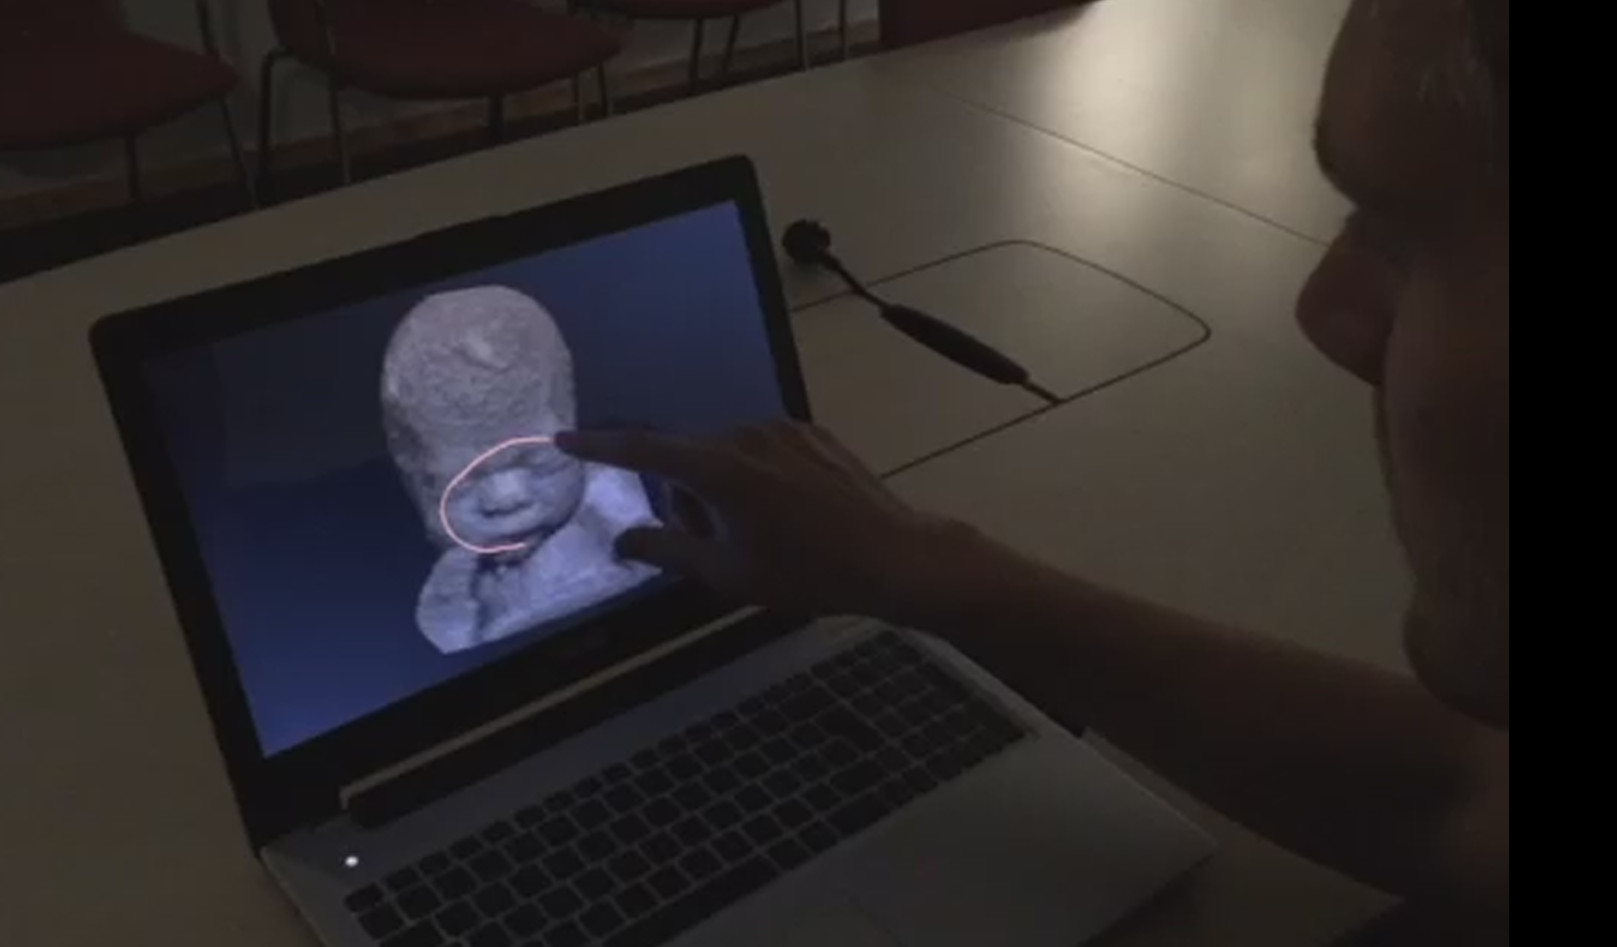
\includegraphics[width=1.0\linewidth]{images/touch_workstation}}
	\caption{Visualization of a fetus scanned using ultrasound. Touch screen interaction is used to change camera, transfer function and clipping.}
	\label{img:touch_workstation}
\end{figure}

\subsection{Presentations in Exhibition Area}
In an exhibition area there is often both small to medium sized displays utilized to showcase and explore the scientific data.
Furthermore, there is mostly none experience users and viewers present which interact and view others interact with the scientific data.
There are a wide range of setups with certain displays and gadgets for immersive and exploratory purposes which can be utilized in an exhibition area, such as \cite{Laha:2013:VCB:2491367.2491368, conf/egve/KruszynskiL08}.
What they all have in common when it comes to this scenario is that naturalness of the interaction is highly important, as their will be many none experienced users using the interaction techniques.
That fact, together with a reasonable level of functionality motivates the usage of hands-only setup, through direct touch \cite{Klein:2012:DSD:2322389.2322403} and touchless methods \cite{O'hara:2013:NTP:2442106.2442111}.

In figure \ref{img:exhibition_table} we see an exhibition setup example, known as an autopsy table \cite{LRFPY11}, where data such as a CT scan of a human can be explored in a close to true scale environment, using direct touch and multi-touch gestures.
Rotation of the object is done with a one finger through an up and down movement, translation is performed with a one finger side-to-side sweeping and zoom with a two-finger pinch gesture.
Various 2D icons are rendered around the visualization for switching states and presenting relevant information about the data.
There are also gripping points for change clipping and transparency level within the visualization.

In a sense it is just an increased version of a tablet, but suitable for a larger audience, as the area surrounding the table is significantly larger.
However, the larger the touch display surface is, the more the presenter has to move around.
With this in mind, the naturalness of the interaction for the user would benefit from as close to real life movements as possible, to support the true scale visualization.
This is of course a challenge for direct touch displays, as there is a 2D instead of a 3D user experience.
However, it can be considered a commonly known practice how to interact with touch displays, through common gestures such as pinch and swipe.
As high-resolution accurate touch screens are available today, this type of setup is very appreciated for both the user and the audience.

\begin{figure}[htb]
	\centering
	\fbox{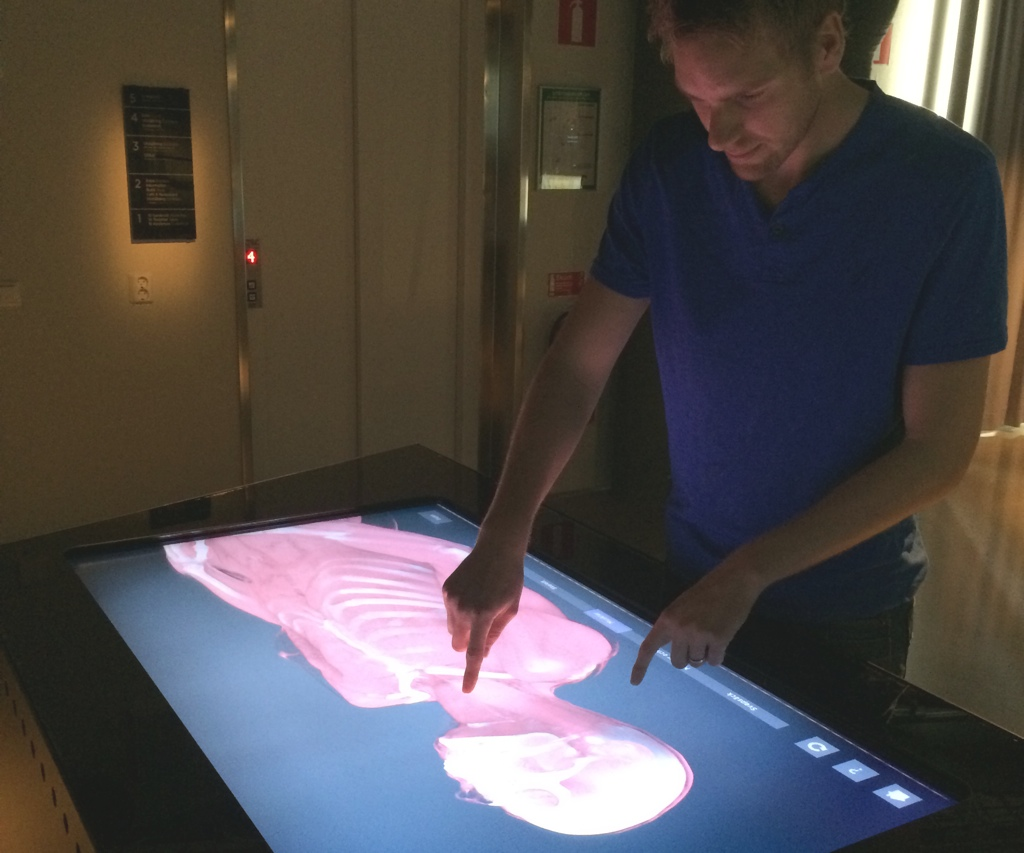
\includegraphics[width=1.0\linewidth]{images/exhib_table}}
	\caption{A touch table (known as the Autopsy Table) for scientific data presentation of, for instance, scans of humans or animals which can be viewed in close to true scale.}
	\label{img:exhibition_table}
\end{figure}

The setup in figure \ref{img:exhibition_kinect} is similar to figure \ref{img:exhibition_table} in terms of exploring data in true scale.
However, we now have a display surface without direct touch, which is instead coupled with hand tracking.
The visualization is also supported by state icons, which is this case determine either a 3D dataset of a bear, moose or penguin is loaded.
Furthermore, a hand cursor is rendered onto the screen which correspond to the projection of the right hand onto the screen \todo{Develop this further in Large Audience section with the rendering of 3D arms....}.
The left hand is utilized to switch to different states such a camera or light source interaction.

\begin{figure}[htb]
	\centering
	\fbox{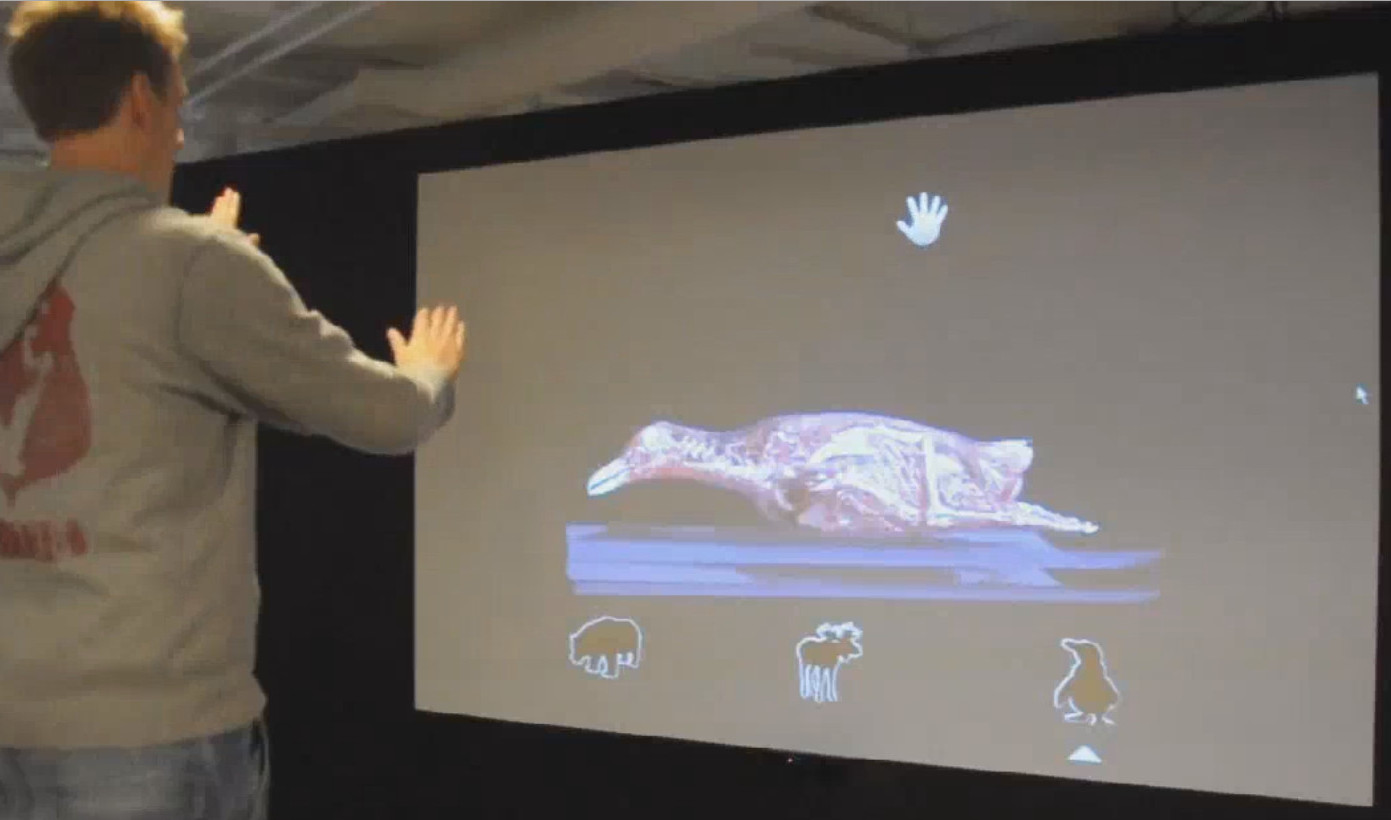
\includegraphics[width=1.0\linewidth]{images/exhib_rotate_peng}}
	\caption{Volume visualization of a CT scanned penguin displayed on a wall with a in-front projector and coupled with a kinect for 3D interaction possiblities.}
	\label{img:exhibition_kinect}
\end{figure}

\subsection{Scenario: Large Audience Presentation}
\noindent \textbf{Oral Presentation} Being the most traditional form of presentation techniques, oral presentations have been around since time immemorial.
While they were limited to a lecturer talking initially, tools and techniques have been added to improve this presentation mode.
A prime example of an enhancement, in which the interaction technique matters a great deal, is medical schools' education based on the dissection of cadavers in class.
Here, not only the presented content is important, but even more important is the way the lecturer interacts with the body.
A limitation to this technique is the fact that every audience member has to see the presenter and cadaver.
We found that this simple restriction is present in many interaction techniques that we investigated, as being able to see and understand the movements and gestures of the presenter is important for the audiences' understanding.

An extension of these techniques are large-scale, large-audience displays showing interactive, rather than predetermined, computer-generated content.
Principally, we can distinguish two classes of solutions for this interaction problem.
%
The first class, being direct interaction, requires the presenter to perform the interaction himself.
The availability for this kind of interaction is heavily dependent on the screen-size and the layout of the venue and resembles the scenario described previously regarding exhibition areas.
%
The second class is indirect interaction (see Figure~\ref{img:dome_presentation}), where the presenter is communicating orally with an entity controlling the visualization.
This means that the voice input itself becomes an interface device between the presenter and the content.
For our argumentation, there is no difference if the presenter is communicating with a second person steering the visualization, or an advanced voice-recognition system.
From the audience's point of view, the presenter is the user of the system and the voice is the interaction technique, and the audience does not know (or care) what happens afterwards.

%From an interaction point of view, this interplay between presenter and controller has both benefits and drawbacks.
%One benefit is the dynamics between the presenter and the controller, creating a more engaging environment for the audience, itself sparking more interaction between the audience and the presenter.
From an interaction point of view, the audience is witness to the intended action of the interaction, rather than the physical act of interacting itself.
The audience knows that, for example, the focus will be on a specific part of a rendering before it happens.
Rather than witnessing the manual interaction leading to that focus, it perceives the interaction as being completely decoupled from the presenter.
By removing any signs of a physical interaction, the presenter can focus on the explanations and content rather than multitasking with the presentation and the controlling.
This decoupling is the prime attribute for this class of interaction solutions and whether this is a benefit or drawback depends on the situation to which it is applied.

A slight variant to this is the concept of remote presentations.
In this case, the presenter is not in the same room as the intended audience, but his voice (and possible video footage) is streamed instead.
Regarding the interaction, there is no change as the presenter's interaction with the content was limited to communication and there was no physical input necessary.
The only visible difference to the audience is the missing presence of the presenter in the same room, which might make other, complementary, sources of interaction impossible (such as using laser pointers).
An increase in future presence technologies will further blur the line between a physically-present presenter and a remote presenter.


\noindent \textbf{Screen sizes} In our research facility, we have access to two display devices that bear superficial similarities, but induce fundamental differences in how the interaction with the visualization and interplay with the audience works.

\begin{figure}
	\centering
	\fbox{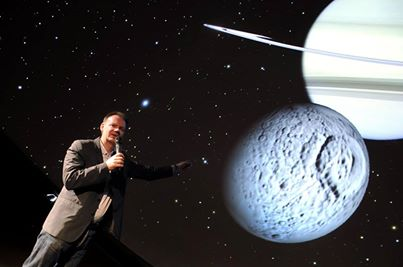
\includegraphics[width=\linewidth, height=165pt]{images/dome_oralpresentation}}
	\caption{Presentation on large scale surfaces using the voice as an interaction technique to communicate intent rather than direct actions.}
	\label{img:dome_presentation}
\end{figure}

One of the display systems is a wide field-of-view hemispherical dome surface with seating for 99 audience members (see figure~\ref{img:dome_presentation}).
This is a similar setup to traditional planetariums, but in our case, the content is produced using an interactive rendering system.
The interaction characteristics for this setup is that both the audience and the presenter are at a physical distance from the projection surface.
This completely inhibits direct interaction techniques like pointing with a finger or doing gestures that are directly relate to the content's position on the screen.
Instead, indirect techniques must be used, like laser pointers, rendered cursors on the screen, gesture recognition, or oral communication.
One issue with this system is the impossibility of mapping physical gestures to match the visualizations.
Due to the large scale of the room and the wide differences in seating position, it is not possible to place the presenter in such a way that his gestures would seem integrated into the visualization for all viewers simultaneously.

\begin{figure}
	\centering
	\fbox{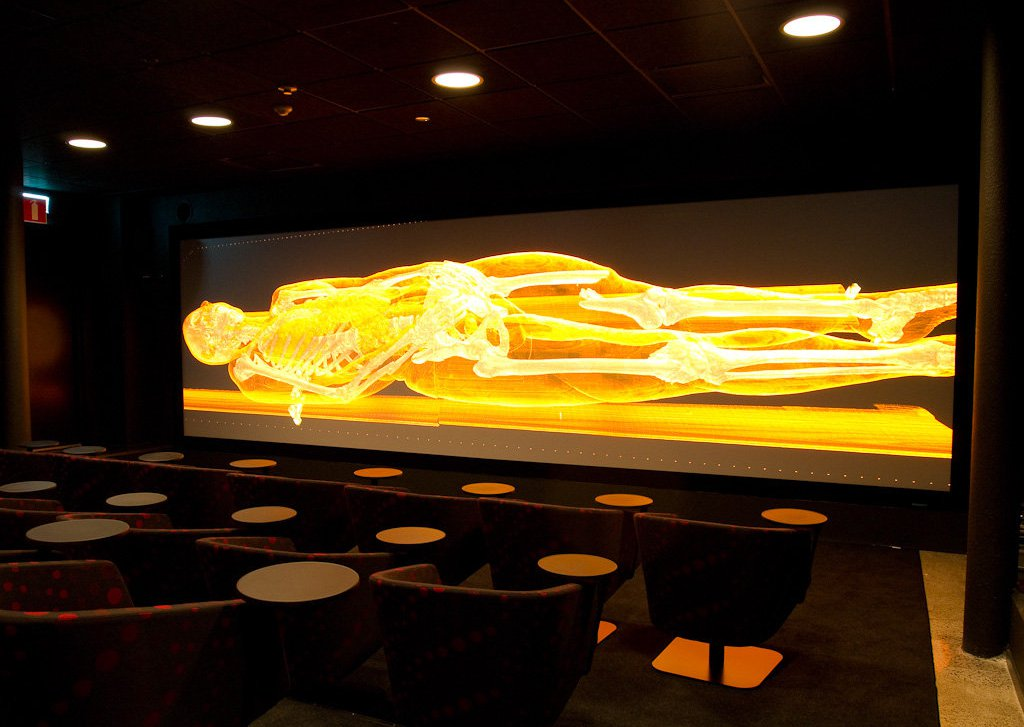
\includegraphics[width=\linewidth, height=165pt]{images/vr_dvr}}
	\caption{A volume rendering on a flat, back-projected surface allowing the presenter direct access to the content.}
	\label{img:vr_dvr}
\end{figure}

The other setup available onsite is a wide, flat, back-projected surface with space for about 30 people (see figure~\ref{img:vr_dvr}).
The benefit of having a back-projection is that the presenter can stand in front of the surface without casting a shadow, thus allowing physical access to the displayed content.
In comparison to the previous setup, this, and the limited size, allows the presenter to walk in front of the whole content and using natural gestures like pointing (which may be integrated, registered, and synchronized with the rendering) to interact with the content.
This natural, gesture-free interaction has been proved very useful in the workflow that we use in the facility.

%The third setup is a curved-screen decision arena in which the audience members are located on the inside of a round room with the walls being used as projection surfaces.
%This setup is very useful for a small group of people ($<$ 10 persons) to simultaneously work on decisions using the information projected on the surfaces.
%The interaction techniques for this, as compared to the previous two, are fairly limited in regular usage, as this is not a tradition presentation setup, but rather a collaborative exploration of data using visualization.



%Presenter is always decoupled from the screen, as the presenter can not interact with the complete presentation surface. This is often due to the lack of touch capability, but foremost the sheer size of common screens for large audience presentations can not be reached from a standing location by the user.

%Dome, movement, viewers benefit to see how presenter interacts with the data.
%Thus, big 3D gestures better then gesture on touch device.

%User should be standing in such away that the 3D movements the user performs can be projected correctly onto the screen.

%Discuss interaction option made by audience, pros and cons


\begin{figure}[htb]
	\centering
	\fbox{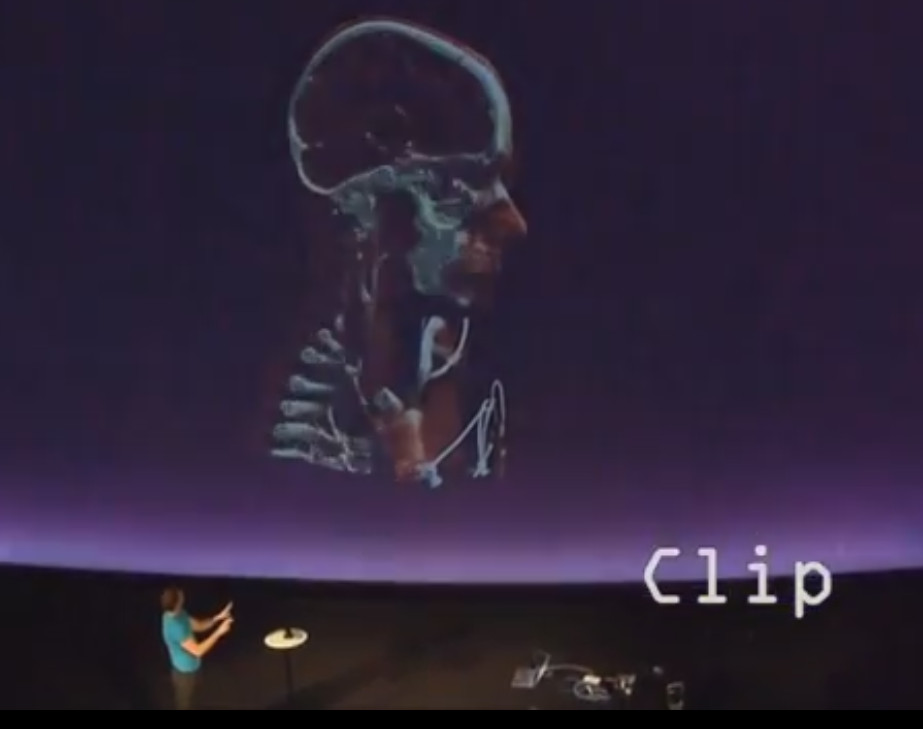
\includegraphics[width=1.0\linewidth]{images/dome_clip}}
	\caption{Dome}
	\label{img:dome_clip}
\end{figure}

%\begin{figure}[htb]
%	\centering
%	\fbox{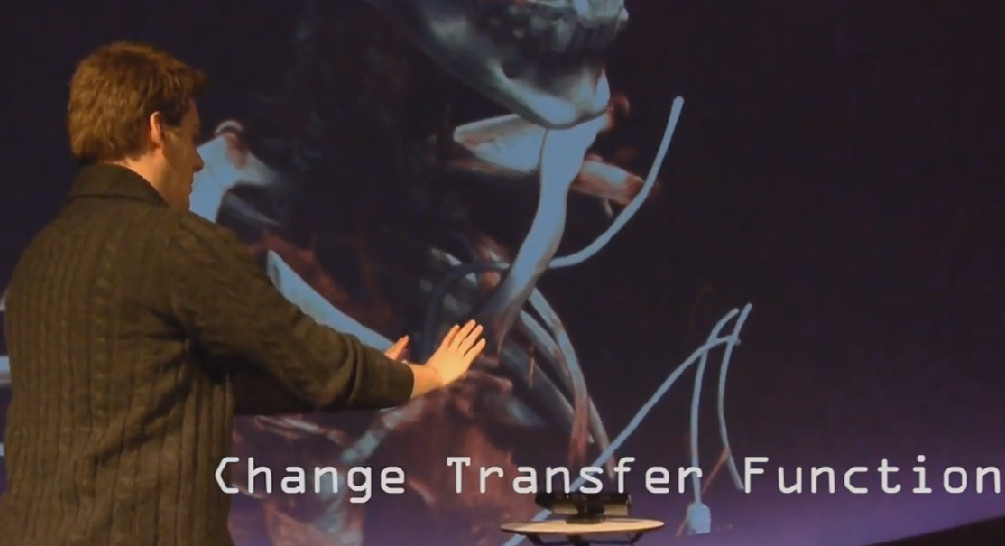
\includegraphics[width=1.0\linewidth]{images/dome_tf_change}}
%	\caption{Dome Closeup}
%	\label{img:dome_tf_change}
%\end{figure}

\section{Interaction techniques from the scenarios} \label{sec:techniques}

So far, not every possible technique suited for the scenarios is covered. However, finding the most suitable technique for our different scenarios is not the focus of our position paper, but rather we propose a way to think about interaction methods dependent on the scenario. In this section we summarize the method of interaction which are part of our previously described scenarios. Furthermore, we discuss there applicability to our scenarios.

\subsection{Direct Touch Interaction}
Direct interaction with an object in the scene gives the user a feel of control of the object~\cite{isenberg2009studying}. 
The user touches the screen and the 2D motion is mapped to a 3D manipulation of the object. 
Touch interaction in scientific visualization has not received much attention in the past \cite{isenberg:hal-00781512}, 
but more work is starting to appear~\cite{Klein:2012:DSD:2322389.2322403} and it has already been used in applications~\cite{LRFPY11}.
This type of interaction is present in scenario 1 and 2, where different sized touch screens are utilized. 
When analyzing this interaction type from a presentation perspective the audience can see the movements of the presenters hands and thereby get an understanding of what will happen on the screen.
Furthermore, there is little distance between the interaction and the display surface and thus spatial related interaction events should be well perceived.
However, the presenter will also hide part of the screen due to the occluding hands and arms. 
When the audience grows larger it may be hard to see the gestures.

%Importance of Touch \cite{Robles-De-La-Torre:2006:IST:1158827.1159097}

\subsection{Touchless Interaction}
Touchless interaction has been found useful in situations such as surgery~\cite{Mentis:2012:IPI:2207676.2208536} where touching an interaction device is cumbersome or should be avoided.
Moving hands freely in the air allows expressive gestures to be created without being restricted to 2D motion as in the case for the direct touch interaction. However, recognizing when a gesture starts and ends can be difficult since there is no natural deactivation state \cite{Kirmizibayrak:2011:EGB:2087756.2087764}. Furthermore, the user/presenter might feel less in control of the data, even if you neglect the accuracy of the tracking, because he is not directly touching the display surface. However, the movements are often expressive and can therefore clearly be seen by the audience during a presentation.

Our scenario 2 includes both a direct touch and a touchless setup, and both setups have been used interactively when presenting scientific data for the same number of people, usually around 10-20. The touchless setup can support a larger audience due the shear placement of the display surface, but comes with the downsides of a decoupled user interaction experience, where the interaction is performed further away from the display surface.

As we evaluate the interaction from an presentation perspective, and how the audience perceive it, we have separated touchless interaction into two categories, registered and unregistered gestures.
We refer unregistered gestures to when the audience see that the presenter is not touching the display directly. 
In contrary, a registered gesture could be touchless if the audience perceive it as it could by a gesture performed directly on the display surface, which is the fact with all gesture on a touch screen.
With that in mind, the most of the audience in the touchless setup in scenario 2 will look upon the display and the gestures performed by the presenter as unregistered gestures.
In a presentation sense, we can easily argue that registered gestures is preferable before unregistered gestures.
 
However, when a decoupled approach is necessary certain elements can be introduced in order to help the audience. As seen in figure \ref{img:exhibition_kinect}, a hand cursor is rendered which simulates the projection of the presenters hand onto the surface. Such visual cues not only help the presenters, but also allow a wider understanding for the audience to comprehend what operation the user is currently expressing, as they can correlate position of the the display to see where the user hand is located in relation to the display.
Furthermore, the icons in the bottom are not only introduced to avoid a increase in the quantity and complexity of gestures for different operations, but also to make the operations performed more in contact with the visualization. To clarify, when the user is moving is hand towards on icon, audience perceive better that something is about to happen, then if the user would perform the same operation through a gesture or a posture \cite{isenberg:hal-00781237}.

However, our observation did show that these elements did bridge the gap between registered and unregistered gestures to an extent that touchless was as suitable as direct touch for an audience size where everyone could see the gestures and the visualization properly on the touch table.

This type of interaction is also present in scenario 3. That type of touchless interaction setup is quite similar, however both the audience size and the display size is now increased substantially. At these display and audience sizes it becomes clear that registered gestures would not be possible, as the presenter could not access the complete display surface with his hands.

Furthermore, seen from a presentation perspective, the touchless gestures in our setup is more expressive then what direct touch gestures on a tablet or a touch table would be. Thus, the touchless setup could be considered as a better presentation tool then utilizing a touch device for remote communication, as done by Coffey et al \cite{Coffey:2012:ISW:2360744.2360843}.

Touching the 3rd dimension \cite{DBLP:journals/dagstuhl-reports/KeefeKSR12}

%Evaluation of Gesture \cite{Kirmizibayrak:2011:EGB:2087756.2087764}

%Discuss gesture vs postures \cite{isenberg:hal-00781237} for kinect, and gesture available for both touch and kinect.

%Mouse vs Kinect vs Leap vs Myo \cite{doi:10.1117/12.2006994}. \todo{I would like to see a paragraph somewhere saying that the actual technology does not matter for the interaction, as there is no big difference between a kinect or a leap motion, for example. (ab)}

\subsection{Voice}

\section{Classification} \label{sec:classification}

To further show when a certain interaction technique is preferable from an expressiveness to audience point of view we introduce a classification of the techniques covered in our scenarios. The chart show the relevance of the technique in relation to audience and display size. It should be noted, that while a technique usage relevance is highly dependent on the scenarios and might be less suitable in when it comes to different scenarios.

\begin{figure*}
    \centering
    \subfigure[Relevance chart mapped to technique categories and our situations.]{
        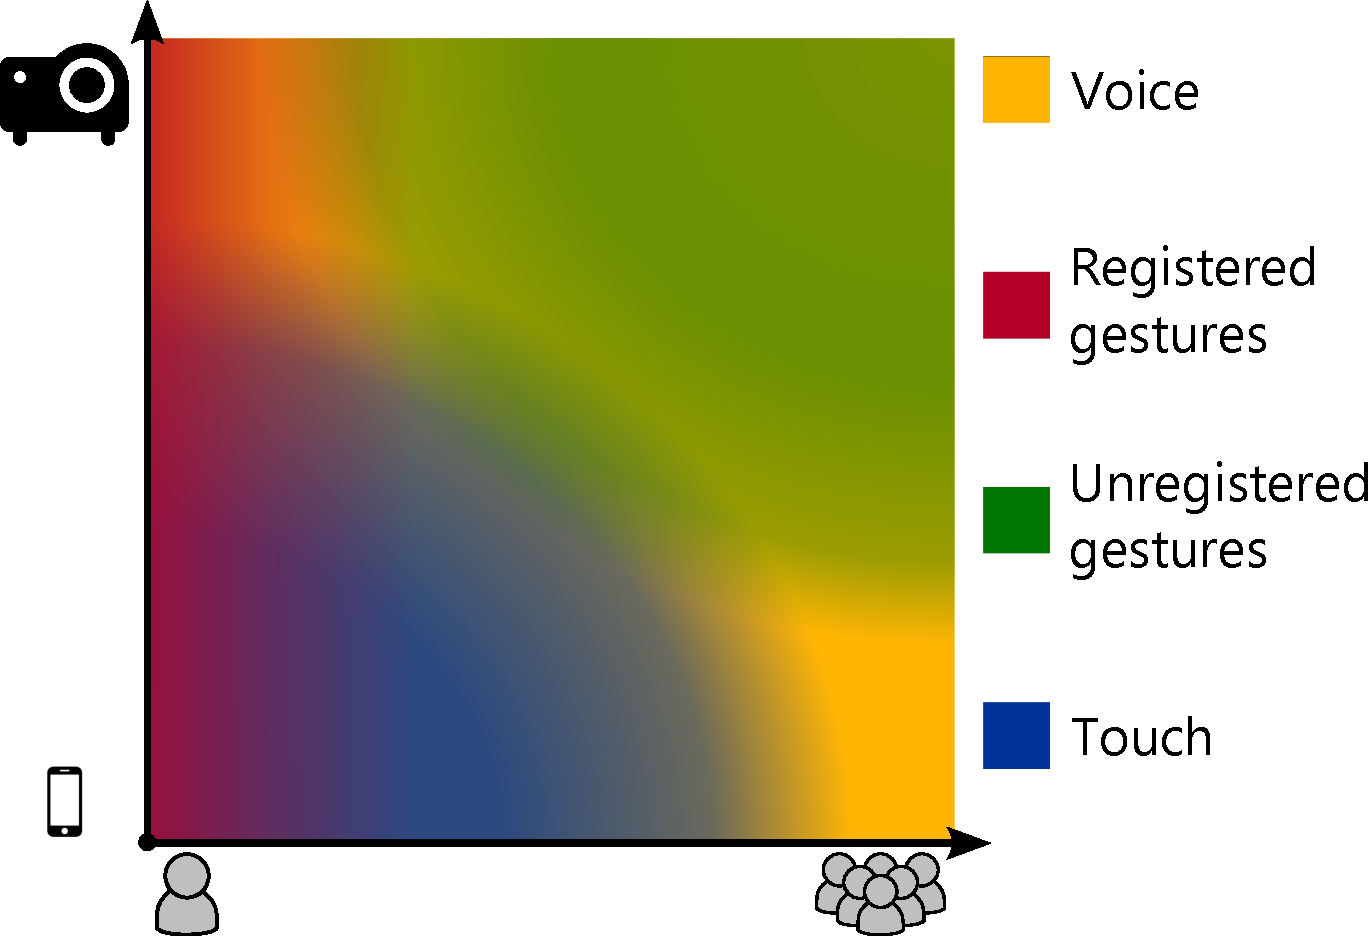
\includegraphics[width=\columnwidth]{classification.pdf}
        \label{classifiy_diagram}
    }
    \hfill
    \subfigure[The ranges of applicability for our chosen scenarios]{
        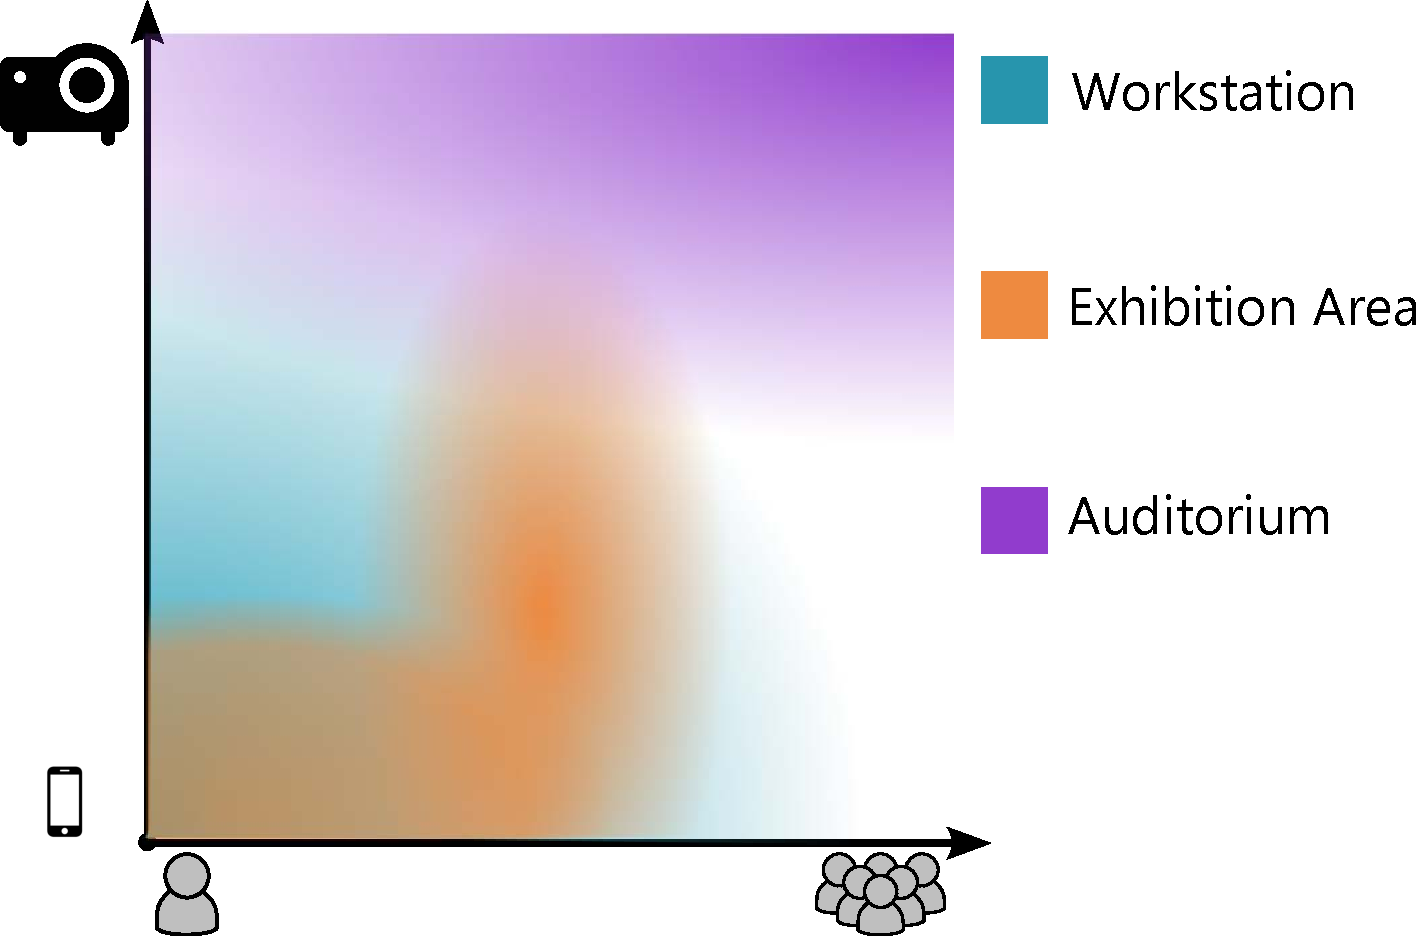
\includegraphics[width=1.0\columnwidth]{expressivity.pdf}
        \label{scenario_diagram}
    }	
\end{figure*}

%\begin{figure}
%	\centering
%	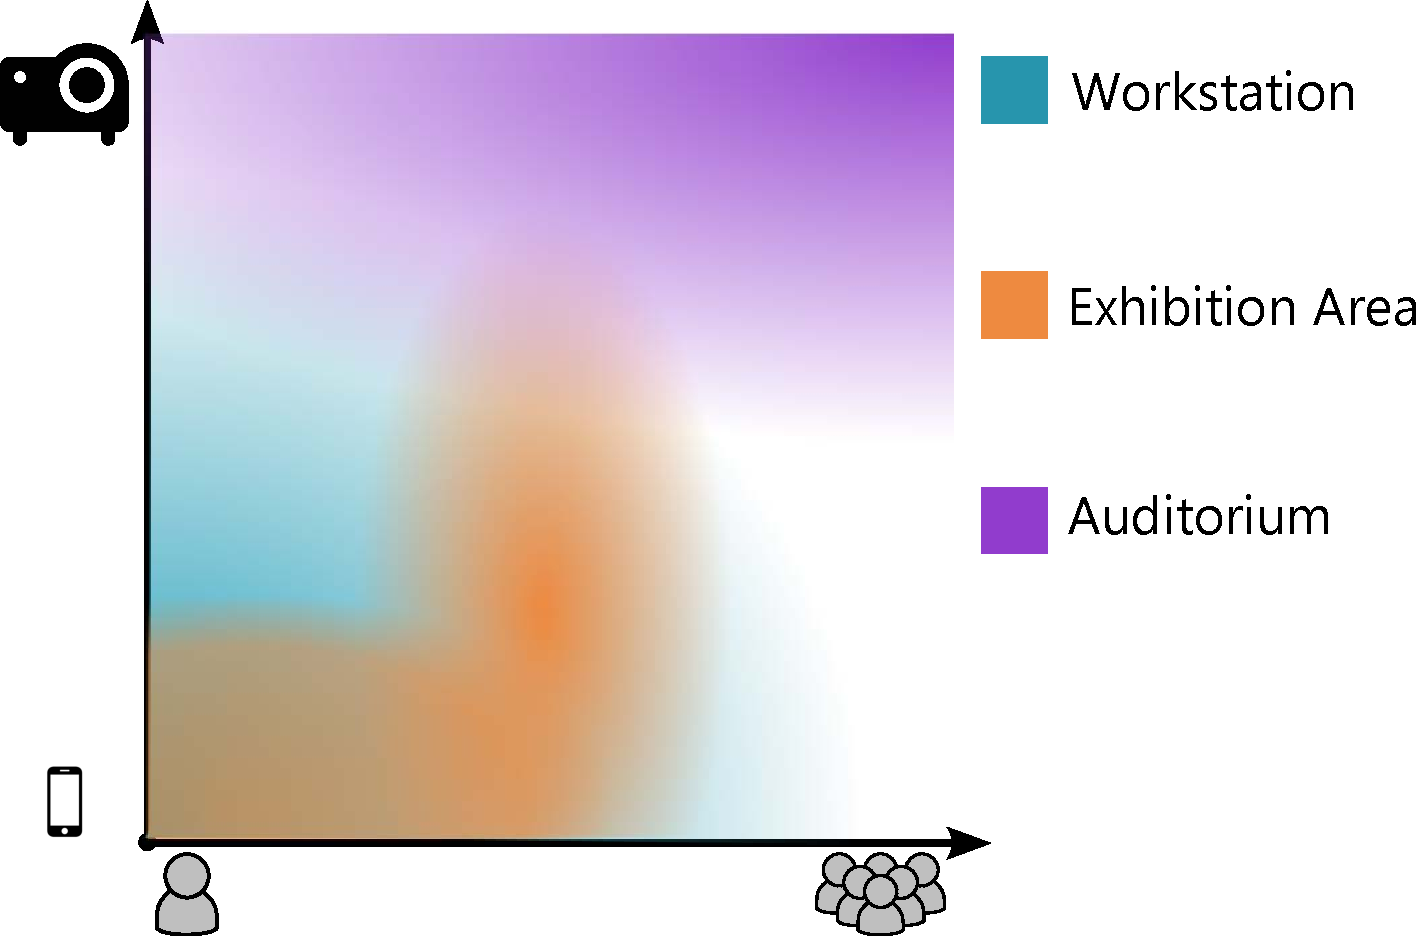
\includegraphics[width=1.0\linewidth]{expressivity.pdf}
%	\caption{The ranges of applicability for our chosen scenarios}
%	\label{scenario_diagram}
%\end{figure}

There are more advanced classification methods for interaction techniques \cite{stars:65-93:2012}, especially for 3D user interaction \cite{CGF:CGF194, Kettner95aclassification, 978-3-319-07458-0_1}, but there focus cover the usability for the actual user.

\section{Conclusions}\label{sec:conclusion}

We have in previous sections detailed presentation scenarios which require interaction and how what are utilized today within these scenarios. As noted, not all interaction methods available are covered, as there are countless others which for instance involve hand-held devices. And in the same aspect, not all scenarios where interaction is suitable is covered. Such as evaluation would be extensive to perform in practice, and as different scenarios change the usefulness of a interaction type, we believe that in order to get as accurate conclusions as possible in an evaluation, only a few interaction techniques per scenario should be compared. Furthermore, showing the importance of different interaction types paired with different scenarios is in our view beneficial for the reason that either new interaction methods or new scenarios could be pre-classified in the current classification we have produced, before a more comprehensive study on suitable interaction for that specific scenario can be performed.

\todo{Emphasize that simple voice commands can be introduced as complementary to 3D tracking to lower the needed complexity of the gestures}

With this paper we wanted to share our observations about interaction as presentation tool and we deem that an the research within viewer or audience centered interaction methods should receive more attention. We strongly encourage researchers within 2D and 3D user interaction interfaces to include this aspect when evaluating previous and future techniques.
Within this subject, expert and none expert viewers have different ways of thinking and experiencing data exploration. Thus, the naturalness of the interaction could does be completely different for various viewers. \todo{Future research to not disclose, exam viewer groups, categories different generations sense on interaction}.

\bibliographystyle{abbrv}
%%use following if all content of bibtex file should be shown
%\nocite{*}
\bibliography{literature}
\end{document}
